%!TEX root = ../template.tex
%%%%%%%%%%%%%%%%%%%%%%%%%%%%%%%%%%%%%%%%%%%%%%%%%%%%%%%%%%%%%%%%%%%%
%% chapter2.tex
%% NOVA thesis document file
%%
%% Chapter with the template manual
%%%%%%%%%%%%%%%%%%%%%%%%%%%%%%%%%%%%%%%%%%%%%%%%%%%%%%%%%%%%%%%%%%%%

\typeout{NT FILE chapter2.tex}%

\chapter{Time Series Fundamentals}
\label{cha:theory}

The content of this thesis is diverse and covers several different topics. Therefore, the reader will appreciate that we set the foundations that are necessary to fully capture the essence of this work. For this, we provide an introduction to each of the topics addressed, the global definitions and used notation in this work. We start by explaining occupational domain variables and corresponding sensors used to monitor these. The data of interest in this work is \textit{time series} and the global definitions and notations are provided. Standard pre-processing methods, representation forms and distance measures are also explained. In this chapter, only global definitions will be made. Each further chapter will have additional and more contextualized definitions when needed.

\section{Global Definitions}
\label{sec:global}

The information gathered by sensors are physical quantities that vary with time. These are called \textit{time series} and are the main topic of this work.


    \item \textbf{Definition 1 - Time Series (T):} A time series is a sequence of real values ordered in time with length $n \in \mathbb{N}$: $T = (t_1, t_2, ..., t_n)$.
    Several domains of data rely in the acquisition of multiple time series from multiple axis of the same sensor (e.g. the 3-axis accelerometer) or from multiple sources (e.g. IMU as a fusion of three different sensors), creating a \textit{multi-dimensional time series}.
    
    \item \textbf{Definition 2 - Multi-Dimensional T (MT):} A \textit{MT} is a set of $k \in \mathbb{N}$ time series belonging to the same acquisition: $\{T_1, T_2, ..., T_k\}$.

Segments of interest are often searched inside a \textit{time series}. A segment is called a \textit{subsequence}:
    
    \item \textbf{Definition 3 - Subsequence (sT):} A \textit{subsequence} is a segment of the time series with size $w \in \mathbb{N}$ and starting from a given position \textit{i} and ending at position \textit{i+w} from the \textit{T} or \textit{MT}. A \textit{subsequence} is delimited by two instants in time. This sample that segments a \textit{subsequence} can be considered an \textit{event}.   
    
    \item \textbf{Definition 4 - Event (E):} Following the definitions of \cite{event_def1, event_def2}, which state that "\textit{an event is a dynamic phenomenon whose behavior changes enough over time to be considered a qualitatively significant change}" and "characterized by an interval of measurements that differs significantly from some underlying baseline", we consider that an \textit{event} is an instant in time \textit{e} that indicates the presence of a relevant occurrence in the time series. Multiple \textit{events} segment the time series into several \textit{subsequences} of different lengths. Therefore, \textit{event} detection is often considered time series segmentation \cite{cpd_alan}.
    
A common strategy used in time series data mining to find relevant \textit{subsequences} or \textit{events} is  the moving window. 

    \item \textbf{Definition 5 - Moving Window (MW):} A \textit{moving window} is a process of sliding along a time series $T$ to apply a specific method on each \textit{subsequence} it hovers. The window has, such as the \textit{subsequence} a predefined size $w \in \mathbb{N}$, which starts at a given position \textit{i} and ends at position \textit{i+w}. The process is iterative and can be made overlapping windows or not. The next window will start at \textit{i+o}, being \textit{o} the overlapping size.

    
With a \textit{MW}, each \textit{subsequence} can be filtered, features can be extracted or distances can be measured. We will show several utilities of this technique further when introducing methods used to pre-process a raw time series and standard distance measures.
\par
Depending on the context and which conditions the data is gathered, the raw information can contain disturbances or should be transformed into another dimension to extract what matters. The set of tasks taken to prepare the \textit{time series} to enhance information retrieval is called \textit{pre-processing}. The pre-processing steps we will discuss involve filtering, normalization and transformation.
\par
After preparing the data, information retrieval techniques are employed, which typically rely on distance measures. In that sense, the standard distance measures are explained. These distances will not only be performed on the numerical domain, but also on the text domain. Therefore, an introduction to the \textit{textual abstraction} of time series will be made in this section as well.

\section{Filtering}
\label{sec:filt}

Time series have multiple sources of disturbance. This disturbance is usually called \textit{noise} and is defined as an unwanted form of energy, but it can have multiple interpretations. It can be caused by internal sources inside a device, such as \textit{white noise}, or be due to external sources, such as motion artifacts, wandering baseline, sensor detachment or the magnetic field from surrounding devices \cite{}. Any of these disturbances will affect the analysis stage and should be detected or removed.

\subsection{Spectral Filtering}
\label{subsec:spec_filt}
Several methods can be used to reduce the influence of noise in the analysis. Standard filtering methods, such as low-pass, band-pass and high-pass filters can be used to reduce the presence of specific frequency bandwidths that are not relevant. There are many configurations for these types of filters, being one commonly used the \textit{Butterworth} filter.

\subsection{Smoothing}
\label{subsec:smooth}

Another often used method that has the purpose of reducing the presence of noise and represents a variation of a low-pass filter is the smoothing technique. Several variations of this technique exist, being the simplest one a moving average, which uses a moving window, calculating the mean in each iteration.

\subsection{Wandering Baseline}
\label{subsec:w_baseline}

Another type of disturbance on the data that is usually removed is a wandering baseline. An example typically occurs in ECG signals, where the respiration creates a wandering baseline on the signal. This type of disturbance has a very low frequency compared to the meaningful information on the data and can be removed by subtracting a \textit{smoothed} version of the original data, or applying a high pass filter.

\section{Normalization} 
\label{sec:normalize}

Normalization of data is an important step in any data mining process. It is essential for data uniformization and scaling, while keeping the morphology and shape of the time series. Several methods can be used for this purpose, namely:

\begin{equation}
\overline{T} = \frac{T}{max(|T|)}
\end{equation}

the normalized signal ($\overline{T}$) is scaled by the absolute maximum of $T$. It is the simplest approach to normalization and guarantees that values are scaled linearly and their modulus cannot be higher than 1.
\par
A variation of this process is the normalization by the range of amplitudes, which is as follows:

\begin{equation}
\overline{T} = \frac{T-min(T)}{max(T)-min(T)}
\end{equation}

here the signal $T$ is normalized to range between [0,1].
Another normalization method, called \textit{z-normalization}, is very commonly used and relies on the distribution of its values:

\begin{equation}
\overline{T} = \frac{T-\mu_T}{\sigma_T}
\end{equation}

where the time series $T$ is subtracted by its mean, $\mu_T$ and scaled by its standard deviation, $\sigma_T$. The resulting values represent how many standard deviations the signal is away from the mean.


\section{Transformation} 
\label{sec:transform}

In information retrieval, data has often to be re-scaled, simplified, approximate or represented into another data type. Each can contribute in their own way to capture the most relevant and meaningful information, or discover a new type of information that once was hidden in the original data. Dozens of methods exist for time series representation, such as Singular Value Decomposition (SVD) or wavelet transform, but only the ones relevant for this thesis will be explained.

\subsection{Spectral Transformation}
\label{subsec:spec_transform}

One of the first and most well known techniques suggested for time series transformation was the Discrete Fourier Transform (DFT) \citep{fourier}. The idea behind this concept is that any signal, of any complexity, is a decomposition of a finite number of sine waves. Each wave is represented by a complex number, known as the Fourier coefficient, transforming the signal from the time domain to the frequency domain \cite{fourier2}. This transformation allows to see the signal in a different manner, highlighting which frequencies concentrate more or less energy. It unveils the presence of specific types of noise or artifacts, or periodic shapes. Figure \ref{fig:fourier} shows the transformation of a signal into the frequency domain.


\subsection{Feature-based Representation}
\label{subsec:features}

\begin{figure}[!h]
\centering
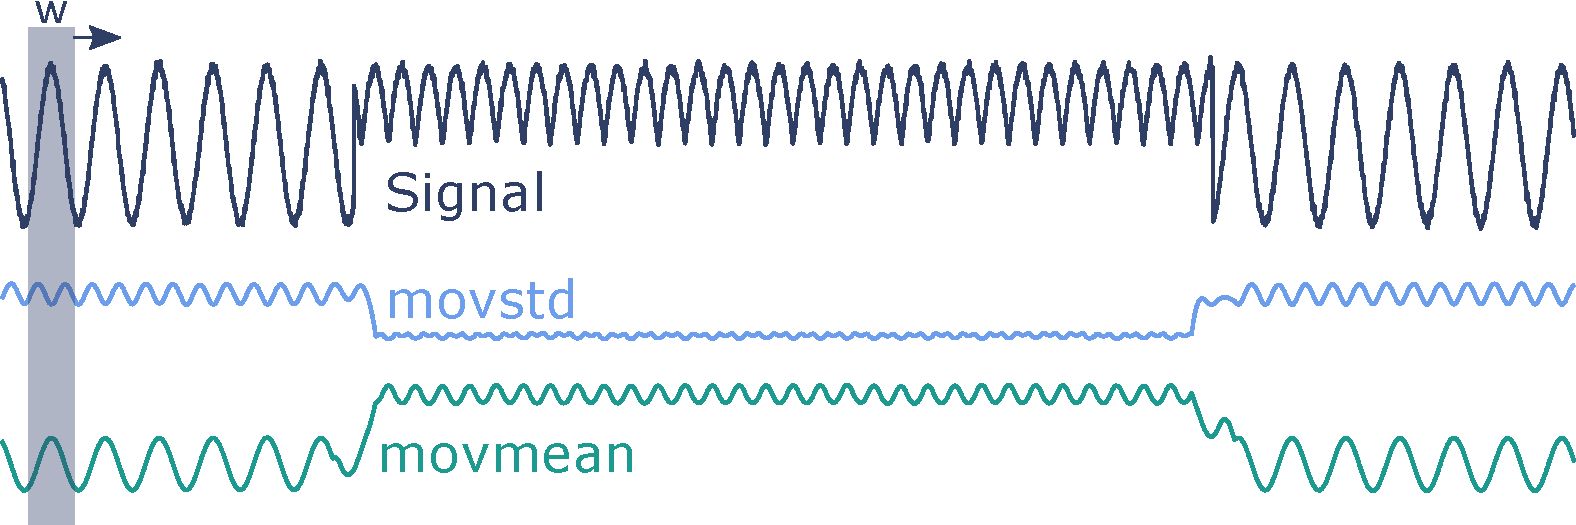
\includegraphics[width=\linewidth]{features.pdf}
\label{fig:feature_intro}
\caption{Moving window used to extract features with total overlap. The mean and standard deviation are extracted from the signal.}
\end{figure}


Frequency properties are very relevant to characterize a time series, but others can also be used to get a full characterization of the signal. The process of feature extraction is also a transformation method commonly employed. It is performed by a moving window from which features are extracted. For each feature, $f$, a feature series is computed.

\item \textbf{Definition 5 - Feature Series (F):} A \textit{feature series}, \textit{F}, is a feature representation of a time series with size $m$ that depends on the overlap size $o \in \mathbb{N}$ of the sliding process, making the size of the resulting feature series $m = \frac{n}{w-o}$. Considering the existence of a MT, the \textit{feature series} becomes a \textit{multi feature series} of stacked \textit{feature series}, with size $f_{k,m}$.
    
When extracting more than one feature, these are grouped into a \textit{feature matrix}.
    
\item \textbf{Definition 6 - Feature Matrix ($F_M$):} A \textit{feature matrix}, $F_M$, is the set of $r$ features extracted for \textit{k} time series, with size $r \times (k\times M)$.
    
On Figure \ref{fig:feature_intro} is showed a time series from which the average (movmean) and standard deviation (movstd) are computed with a moving widow of size \textit{w}=100.   

\subsection{Piecewise Aggregate Approximation}
\label{subsec:paa}

Another common used transformation method to simplify a time series and reduce its dimension is the piecewise aggregate approximation(PAA) \cite{paa}. The new representation space will have size $1 < N \leq n$, in which $N$ is a factor of the original size $n$. The searches to keep the average of the \textit{N} equi-sized subsequences in which the original signal with length \textit{n} is segmented, which results in $\overline{T} = \overline{t_1}, \overline{t_2}, ...,\overline{t_N}$, such that \cite{paa}

\begin{equation}
\overline{t_i} = \frac{N}{n} \sum^{\frac{n}{N}i}_{j=\frac{n}{N}(i-1)+1} t_j
\end{equation}

An example is showed in Figure \ref{fig:paa}, where a \gls{ABP} is converted to \gls{PAA} with sizes 2 and 20, respectively.

    
\begin{figure}[!h]
\centering
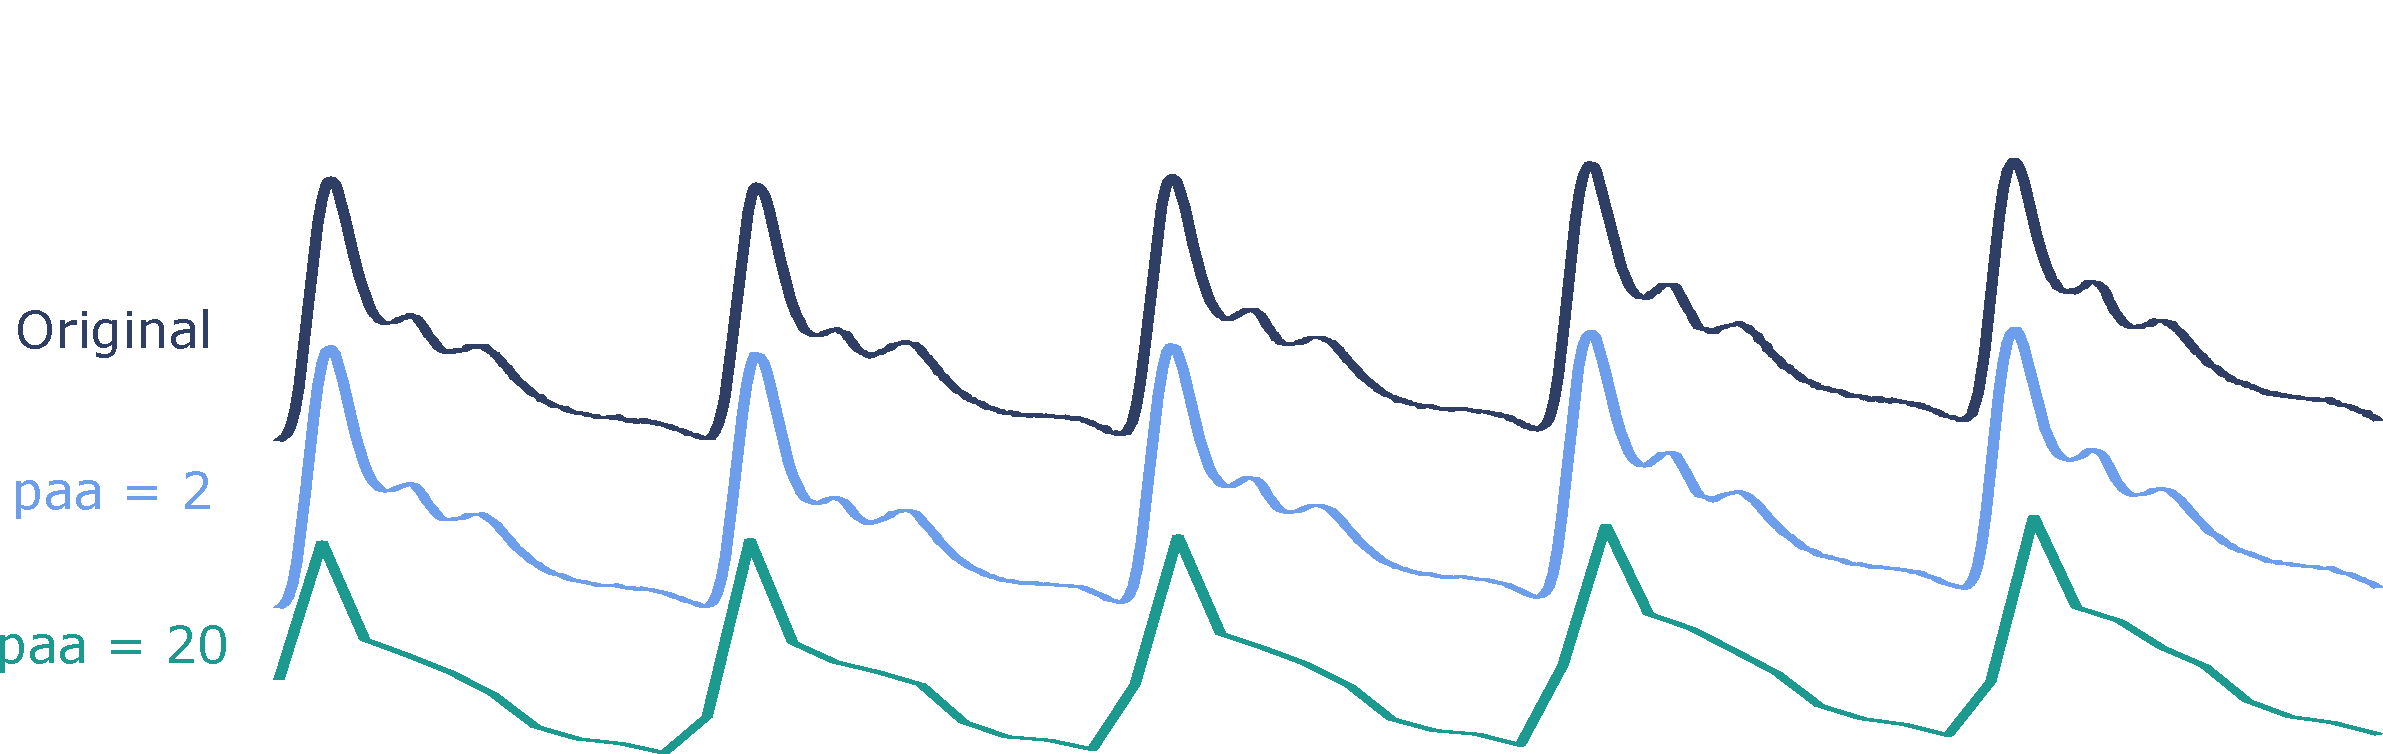
\includegraphics[width=\linewidth]{paa_bvp.pdf}
\label{fig:paa_intro}
\caption{PAA representation of a \gls{ABP} signal, with window sizes of 2 and 20, repsectively.}
\end{figure}
    

\subsection{Symbolic Aggregate Approximation}
\label{subsec:sax}

From this method, a new representation technique was born, transforming the signal from the numerical to the symbolic domain. It is called Symbolic Aggregate approXimation (SAX). This method applies PAA to a z-normalized time series and indexes a \textit{character} to each sample of the simplified signal based on the distribution of its amplitude values. The signal's amplitude values are separated in bins with equal probability. The number of bins is equal to the size of the \textit{alphabet} chosen. Figure \ref{fig:sax} shows an example of the signal transformed into a string with 3 letters in its alphabet. Such as the DFT, SAX opens doors to analyze time series in a completely different manner, profiting from the much acquired knowledge in text mining.

\begin{figure}
\centering
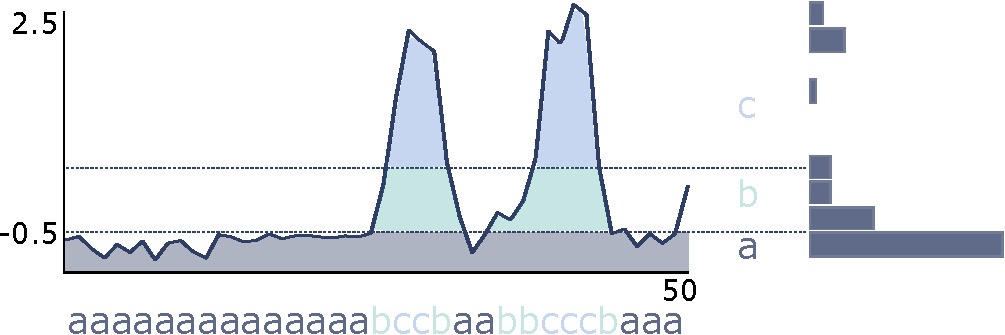
\includegraphics[width=\linewidth]{sax_test.pdf}
\label{fig:paa_intro}
\caption{SAX representation of a power consumption signal from a Dutch Company, with window bin size of 3.}
\end{figure}

In this thesis we will use feature vectors for several purposes. We also propose a novel symbolic representation technique for time series that is used for expressive pattern search and classification. In order to perform search or classification, we have to be able to calculate the difference/similarity between two time series or \textit{subsequences}.

\section{Distance Measures}
\label{sec:distance}

There is an exhaustive number of distance measure for time series, but two of the classical standard measures still provide state-of-the art results in most time series data mining tasks, namely the euclidean distance (ED) and the dynamic time warping (DTW).
\par

\subsection{Euclidean Distance}
\label{subsec:ed}

The ED is the most straightforward distance measure for time series. Let us consider two time series, $Q$ and $C$, of length $n$, so that\\
\\
$Q = q_1, q_2, ..., q_i, ..., q_n$\\
$C = c_1, c_2, ..., c_i, ..., c_n$\\

The distance between these two time series under the ED is:

\begin{equation}
ED(Q,C) = \sqrt{\Sigma^n_{i=1} (q_i - c_i)^2}
\end{equation}

which represents the square root of the sum of the squared amplitude differences between the samples of each signal. Although the distance measure is simple to compute, it is highly susceptible to typical distortions on time series. When using ED, these distortions must be removed, otherwise, other methods, invariant to these distortions, should be used. Examples of distortions are the amplitude and offset distortion, phase distortion, and local scaling ("warping") distortion. The first can be compensated by the z-normalized ED:

\begin{equation}
\label{eq:norm_ed}
z\_ED(Q,C) = \sqrt{2m(1-\frac{\Sigma^m_{i=1}Q_iC_i - m\mu_Q\mu_C}{m\sigma_Q\sigma_C})}
\end{equation}

where $\mu_Q$ and $\mu_C$ are the mean of the time series pair and $\sigma_Q$ and $\sigma_C$ are the standard deviation.

The \textit{warping} distortion can be solved with an elastic measure. For this purpose, DTW is typically used.

\subsection{Dynamic Time Warping}
\label{subsec:dtw}

The DTW distance measures the alignment between two time series. Let us consider two time series, $Q$ and $C$, of length $n$ and $m$, respectively:\\
\\
$Q = q_1, q_2, ..., q_i, ..., q_n$\\
$C = c_1, c_2, ..., c_j, ..., c_m$\\
\\
The alignment is measured by means of a distance matrix with size $n$-by-$m$, where the $(i^{th},j^{th})$ cell of the matrix contains the $d(q_i, c_j)$ between the two points $q_i$ and $c_j$, being $d=(q_i - c_j)^2$ \cite{dtw}. Figure \ref{fig:dtw} shows an example of a distance matrix between two time series. The matrix fully describes the difference between the two time series and maps where these align. The mapping is made by a warping path, $W$, that represent the set of matrix cells that minimize the warping cost, also defined as the cumulative distance of these cells \cite{dtw}

\begin{equation}
W = w_1, w_2, ..., w_k, ..., w_K; \quad \quad max(m,n) \leq K < m+n+1
\end{equation} 

\begin{equation}
DTW(Q,C) = min \sqrt{\Sigma^K_{k=1} w_k}
\end{equation} 

The cumulative distance $\gamma(i,j)$ is calculated as $d(q_i,c_j)$ of the current cell added to the minimum distance adjacent to that cell:

\begin{equation}
\gamma(i,j) = d(q_i,c_j)+min\{\gamma(i-1,j-1), \gamma(i-1, j), \gamma(i, j-1)\}
\end{equation} 

When two time series with the same length have a linear warping path, such that $w_k=(i,j)_k, i=j=k$, we have a special case of the ED. DTW has a time and space complexity of $O(nm)$ while the ED has linear complexity ($O(n)$).
\par
Figure \ref{fig:dtw_intro} shows an example of applying the \gls{ED} and \gls{dtw} on two different PQRS complexes from different \gls{ECG}s. 

\begin{figure}
\centering
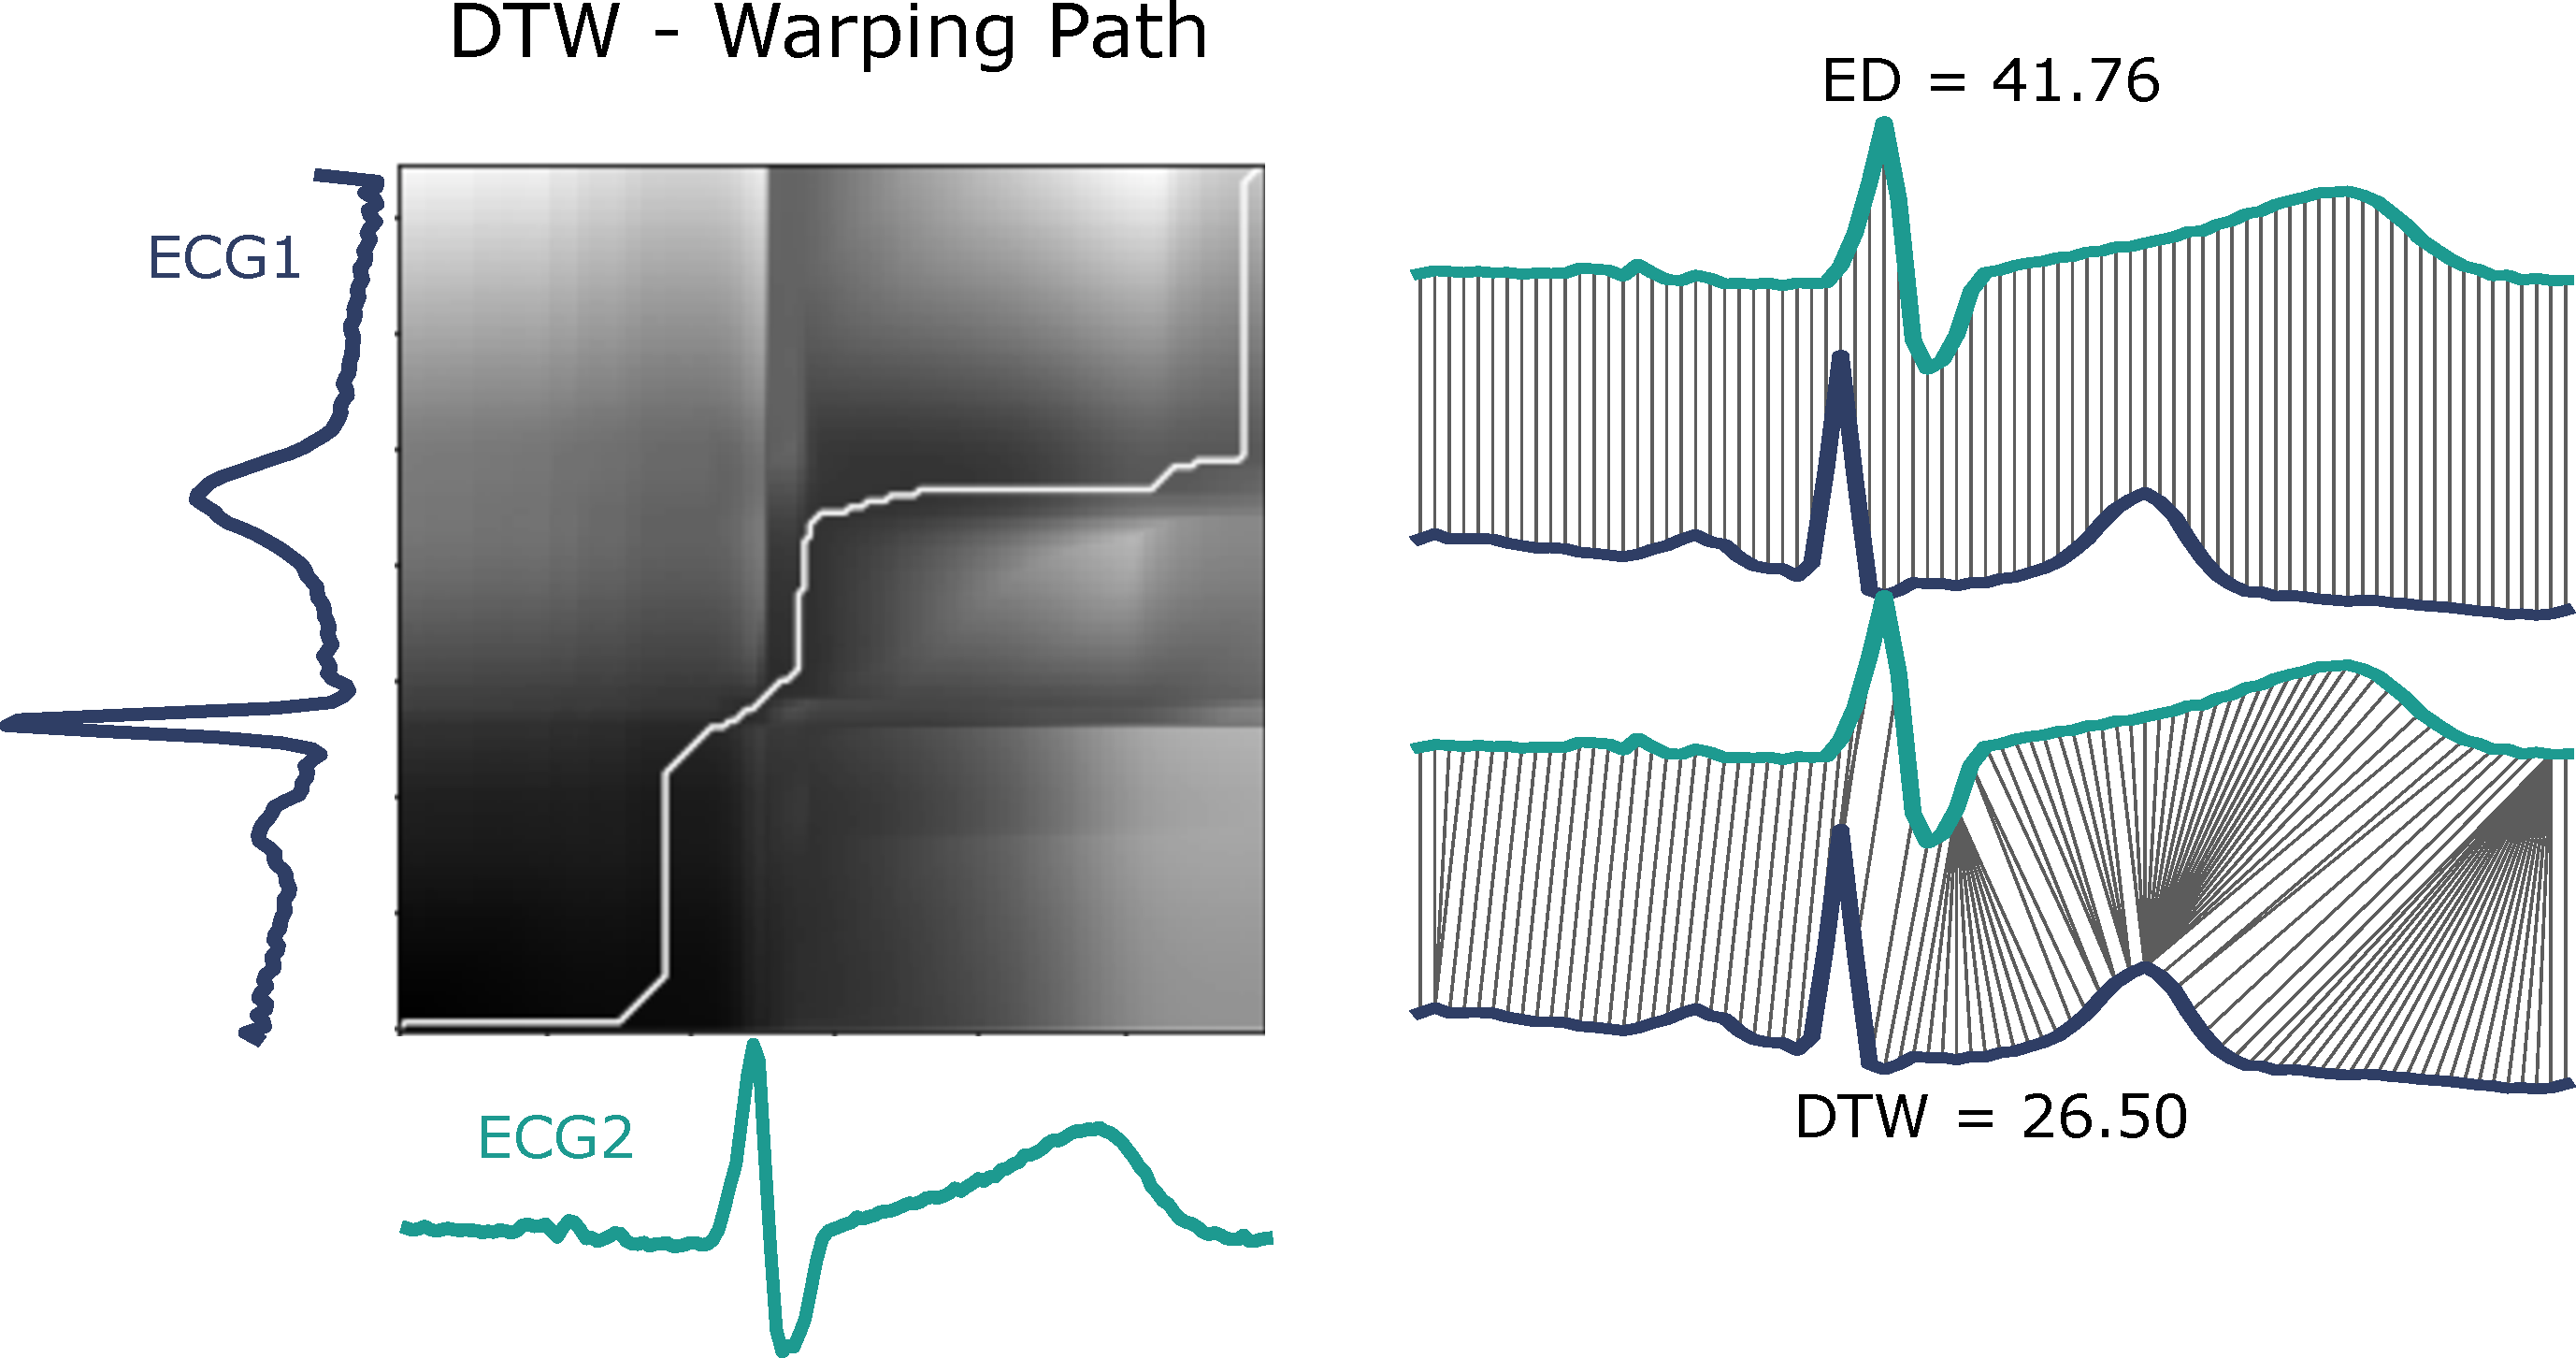
\includegraphics[width=\linewidth]{dtw.pdf}
\label{fig:dtw_intro}
\caption{DTW and ED distances on two different ECG signals.}
\end{figure}

\subsection{Complexity Invariant Distance}
\label{subsec:complexity}

A different type of distance measure is also used to cope with complexity invariance. This distance uses a complexity correction factor ($CF$) with an existing distance measure, such as ED \cite{complexity}:

\begin{equation}
CD(Q,C) = ED(Q,C)\timesCF(Q,C)
\end{equation}

The $CF$ is defined as \cite{complexity}:

\begin{equation}
CF = \frac{max\{CE(Q),CE(C)\}}{min\{CE(Q),CE(C)\}}
\end{equation}

where $CE$ represents the complexity estimate of a time series. This estimate is calculated based on the intuition that if we could  "stretch" a time series until it becomes a straight line, this line would be as long as the complexity of the signal. It can be computed as the sum of the $n-th$ discrete differences along the time series\cite{complexity}:

\begin{equation}
\label{eq:complexity}
CE(Q) = \sqrt{\Sigma^{n-1}_{i=1} (q_i - q_{i+1})^2}
\end{equation}

These distance measures are performed on the original representation domain of time series. As we showed above, other representation techniques can be employed, creating opportunities for other types of approaches. In this work, we explore other representation techniques to create novel ways of exploring time series. Then, we find that the reader will appreciate that we describe other distance measures employed, namely in the feature-based domain. 

\subsection{Feature-based Distance}
\label{subsec:features_dist}

As mentioned, a feature series $F$ can be computed from the original time series to represent it based on a specific feature. If the size of the \textit{moving window} is equal to the size of the time series, than $F$ is represented by a single value. Otherwise, each \textit{subsequence} highlighted by the \textit{moving window} is characterized by the feature and the $F$ is computed as an array. When multiple features are extracted, each \textit{subsequence} is characterized by a set of features, creating a feature vector $\vec{f}$ with $r$ feature values. Vector based distance measures can be used with these feature vectors to compare different time series or \textit{subsequences}. There are several vector-based distance measures, including the already mentioned euclidean distance or the manhattan distance, but we will only describe the cosine similarity/distance.
\par
The cosine similarity is a measure of the angle between two vectors determining if these are pointing in the same direction. Consider two feature vectors $\vec{f_A}}$ and $\vec{f_B}$. Their cosine similarity is computed as their normalized dot product \cite{cosine}

\begin{equation}
CS = \frac{\vec{f_A} \cdot \vec{f_B}}{||\vec{f_A}|| ||\vec{f_B}||}
\end{equation}

being $||\vec{f_A}||$ and $||\vec{f_B}||$ the euclidean norm of each feature vector, defined as $\sqrt{\Sigma_{i=1}^{r} f_{Ai}}$ and $\sqrt{\Sigma_{i=1}^{r} f_{Bi}}$, respectively \cite{cosine}.


\section{Applying Distance Measures}
\label{sec:dist_measures}

Measuring distances between any time series gives the ability to compare them. It is the fundamental instrument for most time series data mining tasks. With a distance measure, we are able to compare groups of time series for classification purposes or compare \textit{subsequences} with a query template and find if it occurs in the time series. Another relevant application of distance measures is its usefulness to retrieve relevant structural information of a time series by comparing each of its \textit{subsequences} to all other \textit{subsequences}. In this subsection, relevant methods applied with the help of the presented distance measures are explained to retrieve information from a time series. We will start with distance/similarity matrices.

\subsection{Self-Distance Matrices}
\label{subsec:dist_matrix}

A time series can reveal relevant information when each \textit{subsequence} is compared to all the other \textit{subsequences} of the same time series. The result is a pairwise distance matrix that unveils \textit{homogeneity}, \textit{repetition} and \textit{novelty} on the time series. Each are relevant assets for segmentation and summarization tasks.
\par
Let $X$ be a sequence with size $N$ that can be a time series or a representation of a time series in the \textit{PAA} or feature space, such that $X = (x_1, x_2, ..., x_i, ..., x_j, ..., x_N)$. Each element of $X$ can either be a single value or a vector with $r$ features. Independently of that, a matrix $S$ with size $N \times N$ can be computed, such that:

\begin{equation}
S(i,j)= d(x_i, x_j) 
\end{equation}

being $d$ a distance measure between elements $x_i,x_j \in X$ for $i,j \in [1:N]$. $S(i,j)$ represents a cell of $S$ that contains the distance value. When $i=j$ the distance should be zero, therefore the diagonal of $S$ has the lower values. Besides the main diagonal, other relevant structures can be found in $S$. These include \textit{homogeneous blocks} and \textit{paths} \cite{fmp, muller}. 
\par
Areas with lower distance are highlighted as \textit{homogeneous} structures. These give an indication of \textit{homogeneity} and \textit{novelty}. \textit{Homogeneity} because a \textit{block} along the diagonal means that the time series has a constant behavior during the segment delimited by the \textit{block}. \textit{Novelty} because when $S$ has multiple \textit{blocks} along the diagonal, it shows that the time series shifted its behavior/regime. The moment there is a transition between \textit{blocks} is a potential segmentation point.
\par
When the time series has repeating \textit{subsequences}, \textit{paths} show up on $S$. The reason for it can be illustrated with the mentioned \gls{dtw} measure. With \gls{dtw}, the z-normalized euclidean distance matrix between two time series is computed and the optimal path is computed as the final cumulative distance. This \textit{path} is a perfect diagonal if the time series are exactly the same, but can be slightly distorted if these are slightly different. The same type of \textit{paths} appear in $S$ indicating a low distance between two different \textit{subsequences} of the time series.

\subsection{Matrix Profile}
\label{subsec:matrixprofile}

As mentioned from the previous subsection, measuring all the distance pairs of a time series provides the ability to retrieve relevant structural information. Recently, a strategy was proposed to compute a one dimensional distance profile for a time series based on a z-normalized euclidean distance matrix. By keeping the \textit{nearest neighbor} of each \textit{subsequence}, we retrieve the \textit{matrix profile}. The result gives the minimal distance pair of each \textit{subsequence}, meaning that minimum values are \textit{motifs} and maximum values are \textit{discords}.
\par


\subsection{Template-based Search}
\label{sec:query_based_search}

The presented distances can also be used to retrieve a distance profile from a \textit{template}. This type of mechanism belongs to the class of query-based search problems. The process to compute this distance profile involves sliding the template along the signal and applying a distance measure to each iteration. The result should indicate which \textit{subsequences} are more (dis)similar to the used template.
\par


\textbf{In this thesis, we will propose other methods to perform query-based searches on a time series. Instead of using a \textit{subsequence} template, we will be using text patterns. REVER}

\subsection{Classification}

- show dendogram
- explain 1-euclidean nn

\section{Text Mining on Time Series}
\label{sec:text_time}

The representation of a time series into the symbolic domain makes possible the usage of text mining methods to analyze time series. The reader will appreciate that an association regarding time series and text is made, and are also introduced relevant methods from the text mining domain, used in this work.

\subsection{Time Series Textual Abstraction}
\label{subsec:text_abstraction}

In \textit{SAX}, the signal is transformed into a sequence of symbols. For this, each sample of the \textit{PAA} representation is converted into a character, which can then form \textit{words} and \textit{sentences}. Other symbolic representation techniques exist on the literature and this work proposes a novel symbolic representation. In that sense, it is relevant to give the general background that makes this association between the original time series, a symbolic time series and text notation. Note that this is an introductory explanation that will be further contextualized when needed throughout this thesis on the corresponding sections.

\item \textbf{Definition 8 - Character (Char):} A \textit{character} is an unit symbolic element that represents a sample or \textit{subsequence} of a time series. Each sample of a time series is transformed into a \textit{character} to form a \textit{symbolic time series}. Sequences of characters form \textit{words}.

\item \textbf{Definition 9 - Symbolic Time Series (ST):} A \textit{symbolic time series} is a sequence of \textit{characters} ordered in time with length $n \in \mathbb{N}$: $ST = (st_1, st_2, ..., st_n)$. A specific sequence of \textit{characters} of a $ST$ can form a \textit{word}.

\item \textbf{Definition 9 - Word (W):} A \textit{word} is the concatenation of a sequence of \textit{characters}, giving a textual representation of a \textit{subsequence}. Putting \textit{words} together forms a \textit{sentence}.


\item \textbf{Definition 10 - Sentence (S):} A \textit{sentence} represents a group of \textit{subsequences}. It is formed by joining sequences of symbolic \textit{words}.

\item \textbf{Definition 11 - Document (D):} The set of \textit{sentences} in a time series are called a \textit{document}. It represents the entire time series.

\item \textbf{Definition 12 - Corpus (GD):} The \textit{corpus} is a collection of text material (group of documents). It represents the higher level of textual information. This collection is typically annotated and used for machine learning tasks. In this case, a corpus will be represented by the set of documents that describe a time series dataset.

\item \textbf{Definition 13 - Vocabulary (V):} The \textit{vocabulary} comprehends the set of all different words present in all time series.

\subsection{Text Features}
\label{subsec:text_features}

From the textual representation, text mining methods can now be applied. Here are introduced traditional methods applied for feature extraction of text data, namely the \gls{bow} and  \gls{tfidf}.

\item \textbf{Definition 14 - Bag of Words (Bow):} A BoW is a feature matrix representation of a corpus, being the feature the number of occurrences of each \textit{term}, called the term-frequency (\textit{tf}):
\begin{equation}
\label{eq:tf}
    bow(t,d) = tf_{t, d} = \frac{f_{t,d}}{\sum\limits_{t'\in d} f_{t',d}}, 
\end{equation}

being \textit{t} the term that exists in a document, \textit{d} the document and \textit{t'} the term that belongs to document \textit{d}. Here $t$ can be a single \textit{word} or an \textit{n-grams}.

\item \textbf{Definition 15} - N-grams: It is a span of followed \textit{words} that are counted in the \gls{bow}/\gls{tfidf}. Possible \textit{2-gram} from Figure \ref{fig:sax} would be \texttt{aa}, \texttt{ca} or \texttt{ac}. This strategy resembles a \textit{moving window} on time series, but for text. It makes the \gls{bow}/\gls{tfidf} model more robust since it makes it rely in more than single \textit{word} statistics. Regarding time series, this method is relevant because it takes into account time dependencies between \textit{words}, which reflects the time dependency seen in time series between \textit{subsequences}.


The \gls{bow} is commonly used to vectorize the textual representation of each symbolic time series, but there is common knowledge in the text mining community that if a \textit{term} occurs in all \textit{documents} it is less relevant. To counteract this limitation, the \gls{tfidf} matrix is used.

\item \textbf{Definition 15 - Term Frequency Inverse Document Frequency (TF-idf):} The \textit{Tf-idf} matrix increases the relevance of $t$ by means of the $t_f$, while reducing its importance in proportion to the number of \textit{documents}, $d$ that contain the term $t$. The model is defined by being a ratio between the $t_f$ and the \textit{inverse document frequency} (idf), which is calculated as follows:

\begin{equation}
\label{eq:idf}
    idf(t, D) = \log{\frac{L}{|\{d \in D: t \in d|\}}}
\end{equation}

\textit{L} is the total number of documents ($L = |D|$). The final equation of the \textit{tfidf} model is the following:

\begin{equation}
\label{eq:tfidf}
    tfidf(t, d, D) = tf(t, d) \cdot idf(t, D) 
\end{equation}

Both \textit{bow} and \gls{tfidf} are matrices that have a vector representation of each \textit{document}, where each element of the vector is the relevance of the \textit{term}. That means that the cosine distance can be used to compute the difference between \textit{documents}.
\par
Due to the probabilistic nature of the \gls{bow} and the fact that it contains discrete features, it is suitable to use in naive bayes classifiers. In the other end, the \gls{tfidf} is typically used with linear support vector machine (SVM) classifiers.

\subsection{Text Pattern Search}

When writing or reading a document, we often have to use the \textit{cntrl+F} key to search for specific words or expressions. This option let us search for direct matches, characters that belong to a word or expression, or even, use \gls{regex}.
\par
The last method is a parsing technique that is convenient to write text patterns, being more flexible than direct matches. It is based on regular languages, following a specific set of rules, and contains a set of meta-characters.
\par
In order to understand the way that regular expressions work, some of the most used characters and \gls{regex} primitives are presented as follows \cite{regex2}:

\begin{table}[!h]
\centering
\renewcommand{\arraystretch}{1.25}
\begin{tabular}{ABC}
\toprule
\textbf{MC} & \textbf{Description} & \textbf{Example of Match}\\
\midrule
\textbf{*} & The preceding item will be matched zero or more times & \textit{eve*nt} $\rightarrow$ [evnt, event, eveent]\\

\textbf{+} & The preceding item will be matched one or more times & \textit{su+b} $\rightarrow$ [sub, suub, suuub]\\

\textbf{?} & The preceding item is optional and will be matched, at most, once & \textit{team?}$\rightarrow$ [tea, team]\\

\textbf{.} & Matches any character & \textit{s.m} \rightarrow [ssm, sam, sim] \\

\textbf{[]} & Matches anything inside the brackets & \textit{wom[ae]n} \rightarrow [women, woman] \\

\textbf{|, \&} & Boolean operators - or, and & \textit{tr(i|a)p} $\rightarrow$ [trip, trap]\\

\textbf{(?=<)} & Positive lookbehind - The string matches the item that is preceded by the pattern inside the lookbehind without making it part of the match & \textit{(?=<http://)} $\rightarrow$ any URL\\

\textbf{(?<!)} & Negative lookbehind - The string matches the item that is not preceded by the pattern inside the lookbehind & \textit{?<!\d*}.+ $\rightarrow$ [\cancel{10th}, th]\\

\textbf{(?=)} & Positive lookahead - The string matches the preceding item that is followed by the pattern inside the lookahead without making it part of the match & \textit{(?=www\backslash .)} $\rightarrow$ matches web protocol\\

\textbf{(?!)} & Negative lookahead - The string matches the preceding item that is not followed by the pattern inside the lookahead & a(?!b) $\rightarrow$ [\cancel{ab}, ac]\\
\bottomrule
\end{tabular}
\end{table}

\subsection{Keyword Extraction}

https://www.analyticsvidhya.com/blog/2018/11/introduction-text-summarization-textrank-python/


\section{Performance and Validation Measures}

In this thesis are mainly discussed three time series data mining domains, namely classification, segmentation and event detection. In order to perform a validation of the work developed, standard procedures are already available. In this section are explained which procedure are typically used to evaluate the performance of algorithms used in these domains.

\subsection{Classification Problems}

(FALTA A ACCURACY)

One of the most common strategies to evaluate algorithms from the machine learning field are \textit{precision} (P), \textit{recall} (R) and \textit{f1-score} (F1). These measures are calculated based on \textit{true positives} (TP), \textit{false positives} (FP) and \textit{false negatives} (FN). Understanding what these metrics represent depend on the problem. These measures are used in this thesis to evaluate the performance of classification and event detection algorithms.
\begin{equation}
\label{eq:precision}
P = \frac{TP}{TP+FP}
\end{equation}

\begin{equation}
\label{eq:recall}
R = \frac{TP}{TP+FN}
\end{equation}

\begin{equation}
\label{eq:f1_score}
F1 = 2 \times \frac{P*F}{P+R}
\end{equation}

In terms of time series classification problems, a labeled dataset with training and testing time series is typically used. The algorithm is trained on the training set and validated on the testing set. In order to perform the validation of the algorithm, the ground truth labels are compared with the labels predicted by the algorithm. This comparison gives the number of \textit{TP}, \textit{FP} and \textit{FN}. 

\begin{itemize}
    \item $TP_c$ - If the label predicted by the algorithm is equal to the target class (positive when positive);
    
    \item $FP_c$ - If the label predicted by the algorithm is falsely classified as the target class when it should not (positive when negative);
    
    \item $FN_c$ - If the label predicted by the algorithm is not labeled as the target class when it should (negative when positive).
    
\end{itemize}

These measures were initially performed in binary classification problems, but can be adapted for multi-classification ones. For this, each class (the target class) is compared to all the other class, being the target class the \textit{positive} and all the other classes \textit{negative}. All measures are calculated for each class. Finally, a macro and micro average of these metrics can be calculated.

\begin{equation}
macroP = \Sigma_{i=0}^c \frac{P_c}{c}
\end{equation}

\begin{equation}
macroR = \Sigma_{i=0}^c \frac{R_c}{c}
\end{equation}

\begin{equation}
microP = \frac{\Sigma_{i=0}^c TP_c}{\Sigma_{i=0}^c TP_c + \Sigma_{i=0}^c FP_c}
\end{equation}

\begin{equation}
microR = \frac{\Sigma_{i=0}^c TP_c}{\Sigma_{i=0}^c TP_c + \Sigma_{i=0}^c FN_c}
\end{equation}

These metrics are typically visualized on a \textit{confusion matrix}, which displays a 2D-map of the ground truth labels VS predicted labels.

\subsection{Event Detection}

Regarding event detection problems, the process involves finding the sample that corresponds to the ground truth event. Considering that it would not be fair to calculate the performance of an event detection algorithm by searching if the ground truth sample is found, we calculate the TP, FP and FN based on an error margin. From these measures, metrics from Equations \ref{eq:precision}, \ref{eq:recall} and \ref{eq:f1_score} are calculated. The estimated events are considered one of the following categories:

\begin{itemize}
    \item $TP_e$ - is counted when the estimated event is in the margin around the ground-truth event;
    
    \item $FP_e$ - is counted whenever it is out of a margin around the ground-truth event, or when there is more than one estimated event inside the margin;
    
    \item $FN_e$ - is counted when there is no estimated event inside the margin of the ground-truth events.
    
\end{itemize}

Additionally, the distance of the \textit{TP} events from the ground-truth events can be calculated with several distance-based metrics, namely the mean-absolute-error (MAE), the mean-squared-error (MSE) and the mean-signed-error (MsE):

\begin{equation}
    MAE = \sum^{k}_{i=1} \frac{|g_{i} - e_{i}|}{k}
\end{equation}

\begin{equation}
    MSE = \frac{1}{k} \sum^{k}_{i=1} (g_{i} - e_{i})^2
\end{equation}

\begin{equation}
    ME = \frac{1}{k} \sum^{k}_{i=1} (g_{i} - e_{i})
\end{equation}

The precision measure is relevant to indicate if the method is able to only estimate events that belong to the ground-truth category, while the recall measure is an important indication of how many ground-truth events are missed in the estimation of the method. Both measures are combined in the F1-measure.
\par
The distance-based metrics evaluate how far are the TP from the corresponding ground-truth events (MAE and MSE) and which is the direction of estimation of events (if before or after the ground-truth events - ME).
\par


\subsection{Comparing Algorithms}

In classification problems, a good procedure is to compare the proposed algorithm with existing state of the art solutions, so that the reader can understand how the results presented are unbiased from the data. In this work, for each strategy proposed in the domains of classification and event detection, we will compare it with existing solutions. There are two typical ways of displaying this comparison: \textit{confrontation maps} and \textit{critical difference maps}, with examples displayed on Figures \ref{fig:performance_plots}.left and \ref{fig:performance_plots}.right, respectively.

\begin{figure}
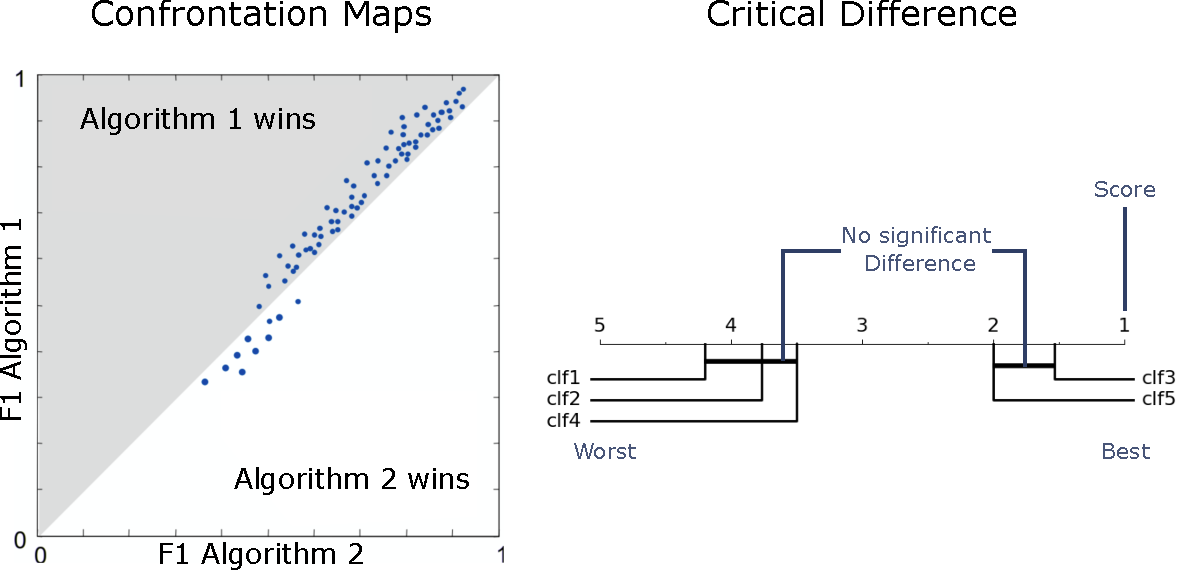
\includegraphics[width=\linewidth]{performance_plots.pdf}
\label{fig:performance_plots}
\end{figure}

\subsubsection{Confrontation Maps}

When the proposed algorithm is applied to a dataset and compared with another algorithm, we might be tempted to display an overwhelming quantity of information in a table. Although this is a valid approach that should be made to give a full picture to the reader, there should also be a straightforward way of displaying the same information but that can be read in a glance. With confrontation maps we can compare the performance of two algorithms just to very intuitively understand if there is a significant difference in their performance. Typically, this map is a scatter plot comparing the \textit{F1-score} or \textit{accuracy} of algorithm 1 \textit{VS} algorithm 2. Figure \ref{fig:performance_plots}.left displays an example of it taken from \cite{keogh_presentation}. Each dot of the plot is a dataset. When it is above the diagonal, it is better classified by algorithm 1, while if below, it is better classified by algorithm 2. In this example, algorithm 1 is better in most datasets.

\subsubsection{Critical Difference}

Critical difference maps are a way of comparing the performance of multiple algorithms or variations of the same algorithm. The plot is a representation of a statistical test over the performance result of each algorithm. The test evaluates if the difference in the performance is significant (critical difference) or not. For instance, on Figure \ref{fig:performance_plots}.right, the plot compares 5 different classifiers (\textit{clf1} to \textit{clf5}) and highlights that the difference in performance is not significant between \textit{clf1, 2} and \textit{4}, neither between \textit{clf3 and 5}. However, \textit{clf3} and \textit{5} have a much better performance than the other classifiers. The closer the classifiers are from the right (1), the better they are. The bold bar connects classifier with performances that are not significantly different.
\par
In this work, we will use an implemented critical difference method from \cite{critical_dif}.
